\documentclass[tikz]{standalone}
\usepackage{amsmath}
\usepackage{amssymb}
\definecolor{bg}{HTML}{171D2B}
\definecolor{aksen}{HTML}{F7B538}
\definecolor{coret}{HTML}{6B7280}
\definecolor{teks}{HTML}{FFFFFF}
\definecolor{hijau}{HTML}{4ADE80}
\pagecolor{bg}
\usetikzlibrary{positioning}

\begin{document}
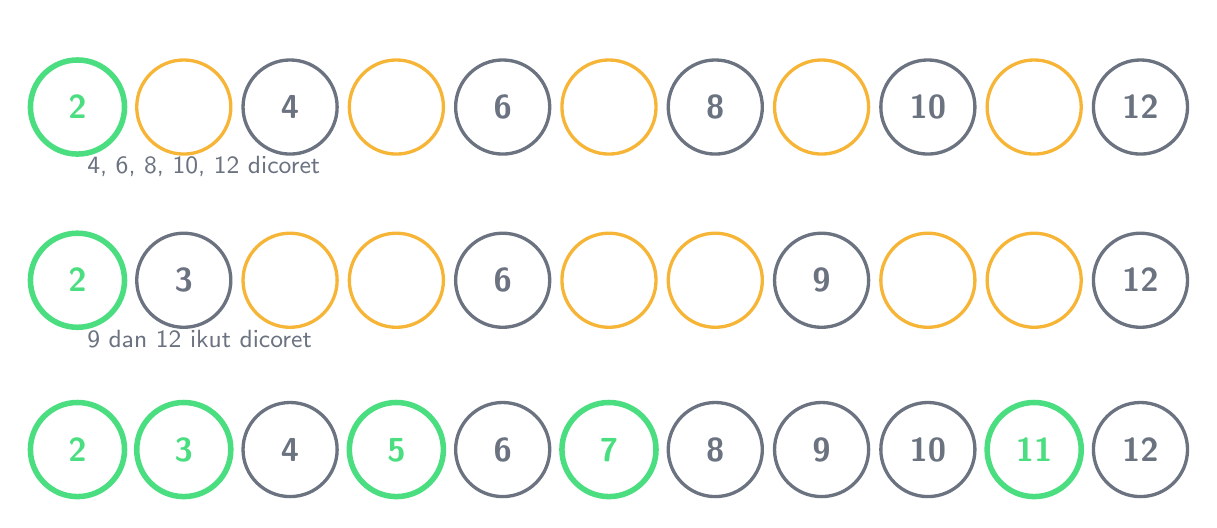
\begin{tikzpicture}[
  ktr/.style={circle, draw=aksen, line width=1.2pt, text=teks,
              font=\sffamily\bfseries\large, inner sep=0pt, minimum size=34pt},
  pr/.style={circle, draw=hijau, line width=2pt, text=hijau,
             font=\sffamily\bfseries\large, inner sep=0pt, minimum size=34pt},
  lbl/.style={text=teks, font=\sffamily\small},
  s/.style={text=coret, font=\sffamily\small}
]

% ===== Panel 1: saringan setelah kelipatan 2 dicoret =====
\node[lbl, anchor=west] at (-7.6,2.35) {\textbf{Langkah 1}: 2 prima, coret semua kelipatannya};
\foreach \n in {2,...,12}{
  \pgfmathtruncatemacro{\r}{mod(\n,2)}
  \ifnum\n=2
    \node[pr] at ({(\n-2)*1.35-7.0},1.6) {\n};
  \else
    \ifnum\r=0
      \node[ktr, text=coret, draw=coret] at ({(\n-2)*1.35-7.0},1.6) {\n};
    \else
      \node[ktr] at ({(\n-2)*1.35-7.0},1.6) {\n};
    \fi
  \fi
}
\node[s, anchor=west] at (-7.0,0.85) {4, 6, 8, 10, 12 dicoret};

% ===== Panel 2: lanjut ke 3 =====
\node[lbl, anchor=west] at (-7.6,0.15) {\textbf{Langkah 2}: bilangan pertama yang tersisa adalah 3};
\foreach \n in {2,...,12}{
  \pgfmathtruncatemacro{\r}{mod(\n,3)}
  \ifnum\n=2
    \node[pr] at ({(\n-2)*1.35-7.0},-0.6) {\n};
  \else
    \ifnum\r=0
      \node[ktr, text=coret, draw=coret] at ({(\n-2)*1.35-7.0},-0.6) {\n};
    \else
      \node[ktr] at ({(\n-2)*1.35-7.0},-0.6) {\n};
    \fi
  \fi
}
\node[s, anchor=west] at (-7.0,-1.35) {9 dan 12 ikut dicoret};

% ===== Panel 3: hasil akhir =====
\node[lbl, anchor=west] at (-7.6,-2.0) {\textbf{Hasil}: bilangan prima sampai 12};
\foreach \n/\done in {2/1,3/1,4/0,5/1,6/0,7/1,8/0,9/0,10/0,11/1,12/0}{
  \ifnum\done=1
    \node[pr] at ({(\n-2)*1.35-7.0},-2.75) {\n};
  \else
    \node[ktr, text=coret, draw=coret] at ({(\n-2)*1.35-7.0},-2.75) {\n};
  \fi
}
\end{tikzpicture}
\end{document}
